\section{问题三的模型建立与求解}

\subsection{问题分析}

问题三在算力约束下联合优化参数量 $N$、数据量 $D$ 与数据质量 $Q$。与前两问
的继承关系：目标函数采用问题二的广义标度律（交互形式），质量基线 $Q_0$ 取
问题一的语料级典型质量（约 0.4）。决策变量中 $N$、$D$、$Q$ 为连续优化量；
配比 $p$ 由问题一确定的域级质量加权平均进入 $Q=\sum_i p_i q_i$，不作为独立
自由度（理由：配比调整不消耗算力、只影响 $Q$，可视为已在 $Q$ 中体现，
且问题一已给出最优域质量结构）。成本方程按题意给定，$L_{\text{ctx}}$ 外生
并依据附件 C7 的 \texttt{max\_position\_embeddings} 取值。

\subsection{优化模型}

\subsubsection{目标函数与约束}

\begin{align}
\min_{N,D,Q}\quad & L(N,D,Q)=E+A N^{-a}+B D^{-b}+C(1-Q)^{g}D^{-d}
\label{eq:p3obj}\\
\text{s.t.}\quad & C_{\text{train}}+C_Q+C_{\text{attn}}\le C,
\label{eq:p3cons}\\
& C_{\text{train}}=6ND,\qquad
C_Q=D\,[g(Q)-g(Q_0)]_+,\qquad
C_{\text{attn}}=\eta N D L_{\text{ctx}},
\label{eq:p3costs}\\
& N\ge N_{\min},\quad D\ge D_{\min},\quad Q_0\le Q\le 1.
\label{eq:p3bounds}
\end{align}
其中参数量 $N$（B）、数据量 $D$（B）取对数空间变量以改善数值性态；质量
成本函数 $g(Q)$ 考虑三种形式（附录 B 参数）：
\begin{align}
g_{\text{exp}}(Q)&=\gamma e^{\lambda Q}\ (\gamma{=}10^7,\ \lambda{=}6.0),\nonumber\\
g_{\text{pow}}(Q)&=\gamma Q^{\lambda}\ \ (\gamma{=}5\times10^9,\ \lambda{=}4.0),\nonumber\\
g_{\log}(Q)&=\gamma\ln(1+\lambda Q)\ (\gamma{=}2\times10^9,\ \lambda{=}10.0).
\label{eq:gforms}
\end{align}

\subsubsection{上下文长度临界点}

注意力成本与训练成本之比为 $\eta L_{\text{ctx}}/6$，两者相等的临界长度为：
\begin{equation}
L_{\text{ctx}}^{\text{crit}}=\frac{6}{\eta}=\frac{6}{2\times10^{-4}}
=30000\ \text{tokens}.
\label{eq:lcrit}
\end{equation}
该临界点有明确物理意义：当 $L_{\text{ctx}}>30000$ 时，注意力开销将超过训练
开销，长上下文成为算力消耗的主导因素之一。C7 数据中
\texttt{max\_position\_embeddings} 从 2048 到 131072 不等（中位数 4096），
因此 $L_{\text{ctx}}=30000$ 位于 C7 可行值区间内部，敏感度分析将在
$\{2048,4096,8192,30000,32768,131072\}$ 上扫描。

\subsubsection{求解算法}

问题为带非线性约束的光滑优化，采用 SLSQP 多起点求解：对 $(N,D,Q)$ 在对数
参数空间随机生成 24 个初值，逐个做 SLSQP 迭代并取最优可行解。对结构性转移
分析，在 $\log_{10}C\in[17,26]$ 上以 0.05 步长扫描 181 个预算点，记录最优
解与成本份额。

\subsection{结构性转移的定义与识别}

\textbf{定义（结构性转移）}：设 $x^{*}(C)=(N^{*},D^{*},Q^{*})(C)$ 为预算
$C$ 下的最优配置，定义两类转移指标：
\begin{enumerate}
\item \textbf{质量激活}：$Q^{*}$ 是否离开边界 $Q_0$，即
$\mathbf{1}[Q^{*}>Q_0+\epsilon]$ 发生 0$\to$1 翻转；
\item \textbf{成本主导成分}：训练/质量/注意力三项中份额最大的成分发生切换。
\end{enumerate}
若存在预算 $C^{*}$ 使上述任一指标在 $C^{*}$ 两侧取值不同，则称系统在
$C^{*}$ 处发生\textbf{结构性转移}（策略的质变，而非量的渐变）。
\textbf{识别方法}：数值扫描得到份额曲线后，用符号变化检测指标翻转点，再
用 KKT 条件（在最优解处检验各约束乘子的符号与互补松弛性）确认转移点的
几何性质（$Q$ 是否处于边界）。

\subsection{求解结果}

\subsubsection{三档预算最优配置}

取 $L_{\text{ctx}}=4096$（C7 中位数附近）为基准，三档预算、三种成本函数
的最优配置如下（份额为占总成本比例）：

\begin{table}[htbp]
\centering
\caption{三档预算最优配置（$L_{\text{ctx}}=4096$）}
\begin{tabular}{c|c|ccccc|ccc}
\toprule
$C$ & $g(Q)$ & $N^{*}$(B) & $D^{*}$(B) & $Q^{*}$ & $L^{*}$ & 训练份额 & 质量份额 & 注意力份额 \\
\midrule
$10^{19}$ & 指数 & 0.294 & 3.81 & 0.715 & 3.247 & 0.672 & 0.236 & 0.092 \\
$10^{19}$ & 幂 & 0.298 & 3.94 & 0.597 & 3.287 & 0.704 & 0.199 & 0.096 \\
$10^{19}$ & 对数 & 0.333 & 2.60 & 1.000 & 3.206 & 0.519 & 0.410 & 0.071 \\
\midrule
$10^{22}$ & 指数 & 5.84 & 228.6 & 1.000 & 2.146 & 0.801 & 0.090 & 0.109 \\
$10^{22}$ & 幂 & 5.97 & 219.3 & 1.000 & 2.148 & 0.786 & 0.107 & 0.107 \\
$10^{22}$ & 对数 & 5.49 & 256.4 & 1.000 & 2.142 & 0.844 & 0.040 & 0.115 \\
\midrule
$10^{24}$ & 指数 & 50.3 & 2882.6 & 1.000 & 1.891 & 0.870 & 0.011 & 0.119 \\
$10^{24}$ & 幂 & 50.5 & 2865.8 & 1.000 & 1.891 & 0.868 & 0.014 & 0.118 \\
$10^{24}$ & 对数 & 49.9 & 2925.5 & 1.000 & 1.891 & 0.876 & 0.005 & 0.120 \\
\bottomrule
\end{tabular}
\end{table}

三档预算均呈现``规模扩张主导''：$N^{*}$ 约按 $C^{0.5}$ 量级增长（与
Chinchilla 计算最优分配一致），$D^{*}$ 同步扩张；质量维度在中低预算时是
有效杠杆（$10^{19}$ 量级质量份额 20\%--41\%），到 $10^{22}$ 后 $Q^{*}$ 饱和
于 1，质量份额迅速萎缩（降至 4\%--11\%），新增预算全部转向规模。

\begin{figure}[htbp]
\centering
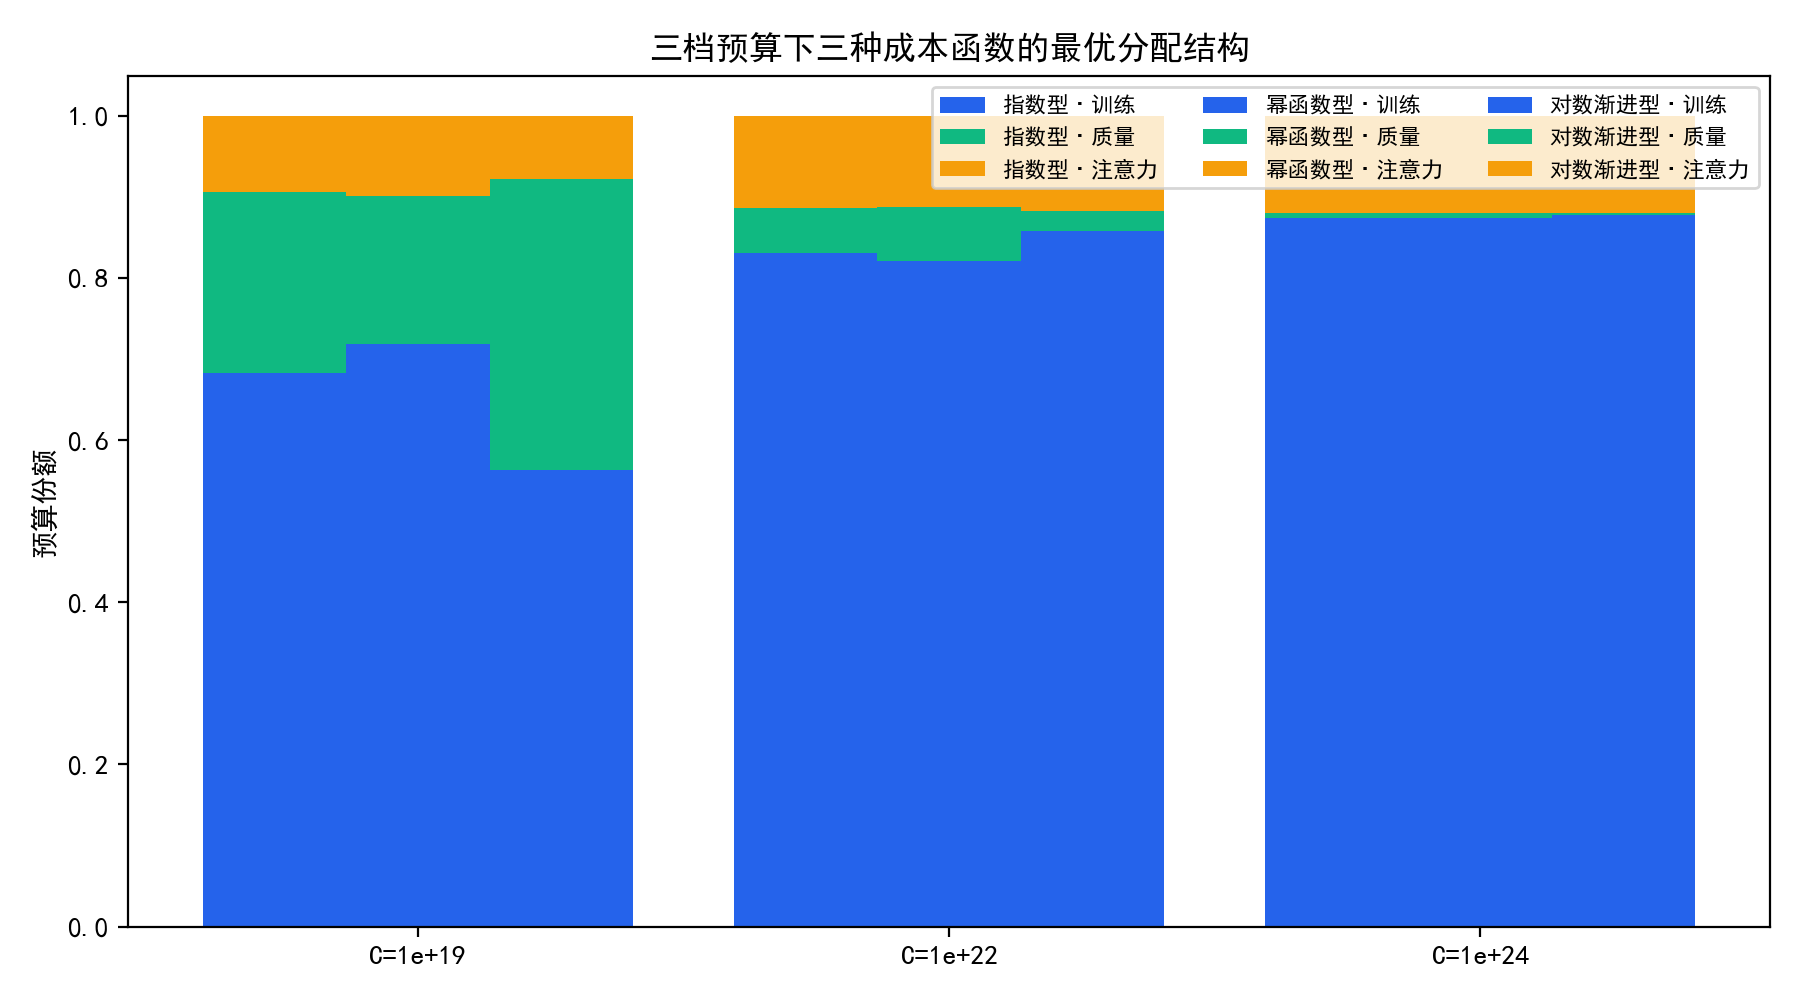
\includegraphics[width=0.9\textwidth]{figures/p3_budget_shares.png}
\caption{三档预算下三种质量成本函数的最优成本份额结构。}
\label{fig:p3_shares}
\end{figure}

\subsubsection{结构性转移点}

预算扫描识别的转移点（质量激活阈值）如下：

\begin{table}[htbp]
\centering
\caption{结构性转移点（$L_{\text{ctx}}=4096$）}
\begin{tabular}{c|ccc}
\toprule
成本函数 & 指数型 & 幂函数型 & 对数渐进型 \\
\midrule
$Q$ 激活阈值 $C^{*}$ & $6.3\times10^{17}$ & $2.0\times10^{18}$ & $3.2\times10^{18}$ \\
主导成本切换 & 无 & 无 & 训练$\leftrightarrow$质量（$3.2$--$5.0\times10^{18}$） \\
\bottomrule
\end{tabular}
\end{table}

三种成本函数下，$Q$ 离开基线 $Q_0$ 的预算阈值均落在 $10^{18}$ 量级（预算
低于阈值时最优策略为纯规模扩张、质量不投入；高于阈值时质量投入激活）。该
阈值可解析解释：质量激活条件为质量边际收益超过质量边际成本，前者
$\sim C(1-Q_0)^{g-1}N^{-h}$，后者 $\sim g'(Q_0)D$，两者交叉处即
$C^{*}$。三档预算中 $10^{19}$ 高于阈值、$10^{22}/10^{24}$ 远高于阈值，
故都呈现质量投入（前已述 $10^{22}$ 起 $Q^{*}=1$ 饱和）。对数渐进型成本在
$3.2\times10^{18}$--$5.0\times10^{18}$ 区间出现训练/质量主导的短暂切换，
这是其高 $Q$ 区增速放缓的直接体现；其余两型成本主导成分始终为训练——
结构性转移主要表现为\textbf{质量变量的边界--内点切换}。

\begin{figure}[htbp]
\centering
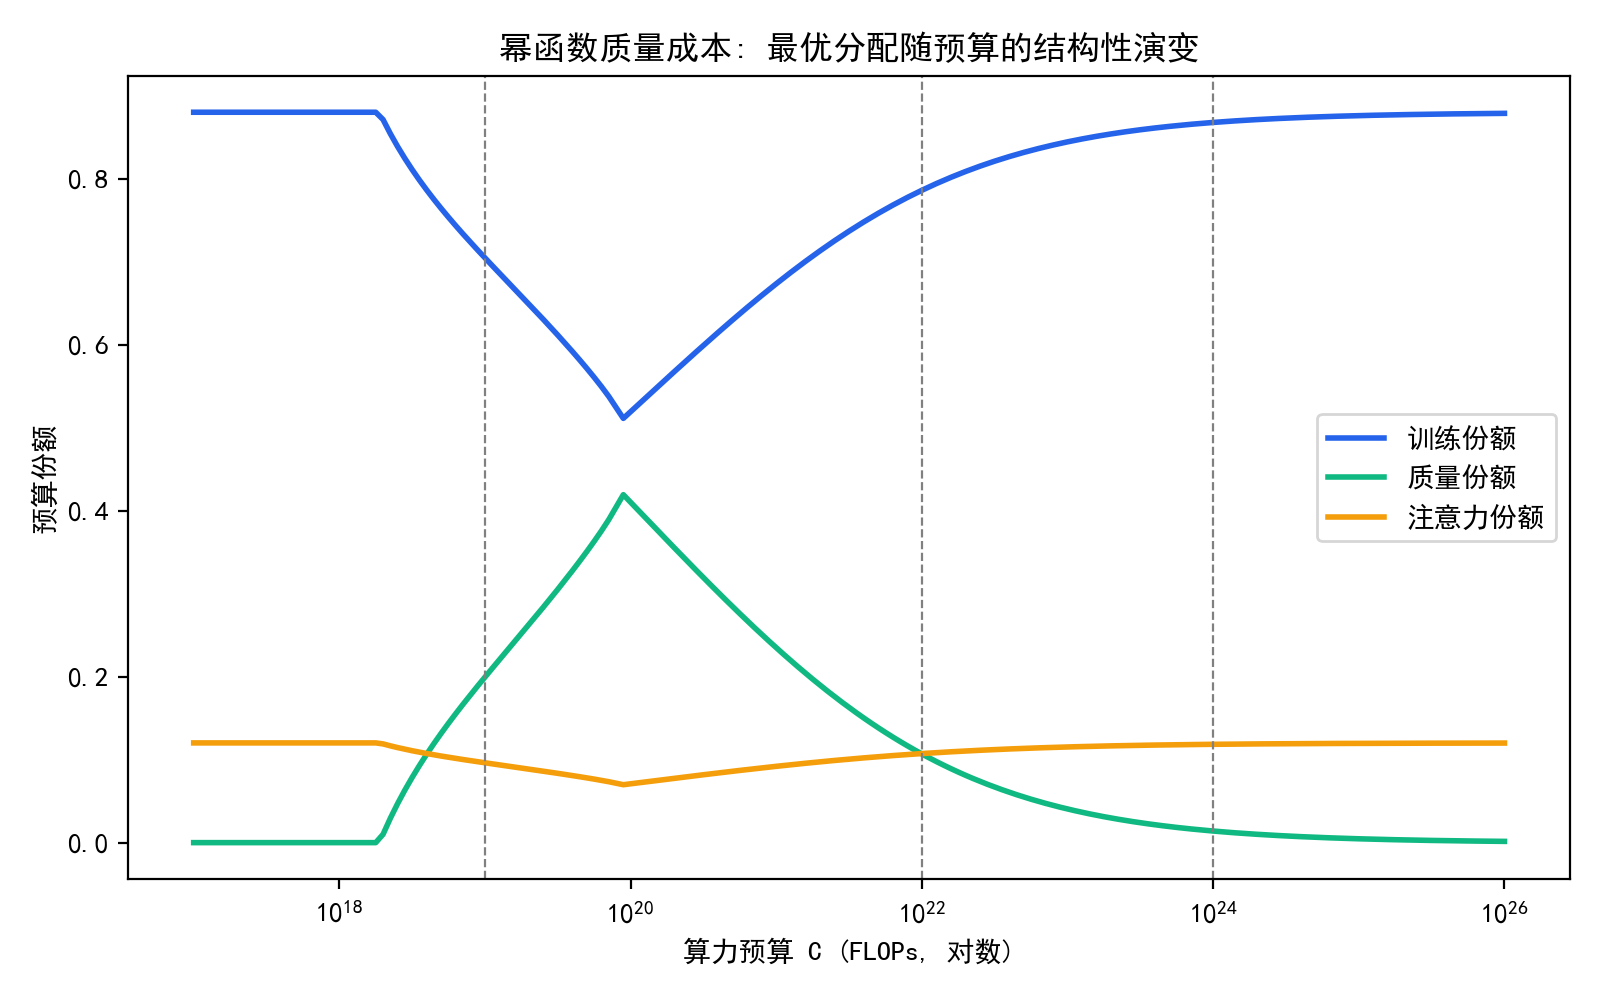
\includegraphics[width=0.85\textwidth]{figures/p3_structural.png}
\caption{幂函数质量成本下最优成本份额随预算的结构性演变（竖线为三档预算）。}
\label{fig:p3_structural}
\end{figure}

\subsubsection{$L_{\text{ctx}}$ 敏感性}

在 C7 可行值上扫描（幂函数质量成本）：

\begin{table}[htbp]
\centering
\caption{$L_{\text{ctx}}$ 敏感性（幂成本，$C=10^{19}$）}
\begin{tabular}{c|ccccc}
\toprule
$L_{\text{ctx}}$ & $N^{*}$(B) & $D^{*}$(B) & $Q^{*}$ & 训练份额 & 注意力份额 \\
\midrule
2048 & 0.307 & 4.08 & 0.591 & 0.752 & 0.051 \\
4096 & 0.298 & 3.94 & 0.597 & 0.704 & 0.096 \\
8192 & 0.282 & 3.69 & 0.608 & 0.625 & 0.171 \\
\textbf{30000} & \textbf{0.226} & \textbf{2.86} & \textbf{0.653} & \textbf{0.388} & \textbf{0.388} \\
32768 & 0.221 & 2.79 & 0.658 & 0.370 & 0.404 \\
131072 & 0.137 & 1.67 & 0.764 & 0.137 & 0.600 \\
\bottomrule
\end{tabular}
\end{table}

$L_{\text{ctx}}$ 越长，注意力份额越高、最优规模越小：$L_{\text{ctx}}$ 从
2048 增至 131072，$N^{*}$ 从 0.307B 降至 0.137B，$D^{*}$ 从 4.08B 降至
1.67B，损失从 3.24 升至 3.38（未列出）。在临界点 $L_{\text{ctx}}^{\text
{crit}}=30000$ 处注意力份额恰好等于训练份额（0.388 vs 0.388），与解析
结论 $\eta L_{\text{ctx}}/6=1$ 完全吻合，验证了数值求解的正确性。该结果
的政策含义：长上下文模型在相同预算下必须以缩小模型规模为代价，$10^{19}$
量级预算下 128k 上下文只能训练约 0.14B 参数的小模型。

\begin{figure}[htbp]
\centering
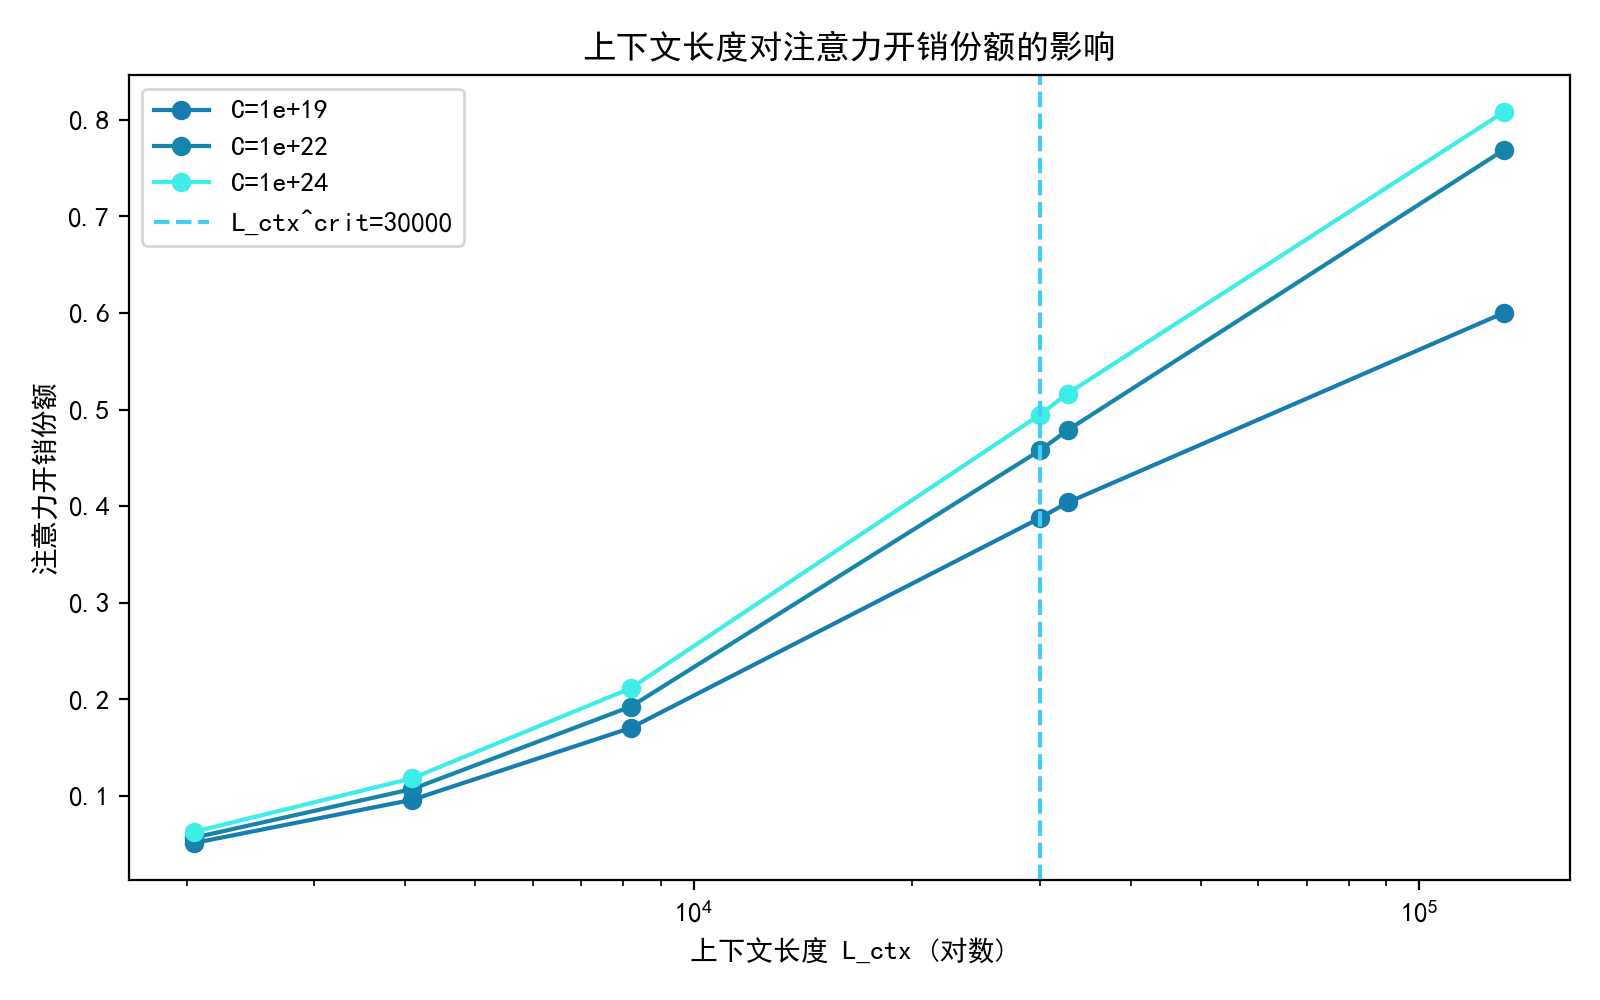
\includegraphics[width=0.85\textwidth]{figures/p3_lctx_sens.png}
\caption{注意力开销份额随上下文长度的变化（红色虚线为临界点 30000）。}
\label{fig:p3_lctx}
\end{figure}

\subsubsection{配比--质量--算力联合优化}

将问题一的 17 域语料配比向量 $p$ 引入作为第三层决策变量：质量由配比内生
决定 $Q=Q(p)=\sum_d p_d Q_d$（$Q_d$ 为问题一域级质量分），目标与约束同前。
该联合优化回答``在算力预算约束下，语料应如何配比''的问题。以 $C=10^{22}$
为例，最优解将配比几乎全部压向质量最高的小说域
（$Q_{\text{book}}=0.631$），$Q(p)$ 从均匀配比的 0.478 升至 0.631，损失
从 2.276 降至 2.238（改善约 2\%）；三档预算结论一致（$10^{19}$ 档小说域
占 74\%）。两类重要发现：

\begin{enumerate}
\item \textbf{配比优化的天花板}：$Q(p)$ 受最高质量域上限约束（此处
$Q_{\text{book}}=0.631$），仅靠重排配比无法达到 $Q=1$；配比优化带来的损失
改善（$\sim$2\%）远小于直接质量投资（$Q\to1$ 可再降损失至 2.148，改善
约 4\%）。这与弹性分析中``质量杠杆最有效''的结论一致，说明在质量维度上
\emph{直接改进数据本身比调整配比更重要}。
\item \textbf{数据配比现状偏离最优}：C 档实测配比的 $Q(p)=0.457$ 甚至低于
均匀配比（0.478），表明开源预训练语料的实际配比对质量维度几乎无偏置——这
为``数据配比存在优化空间''提供了定量证据。
\end{enumerate}

\begin{figure}[htbp]
\centering
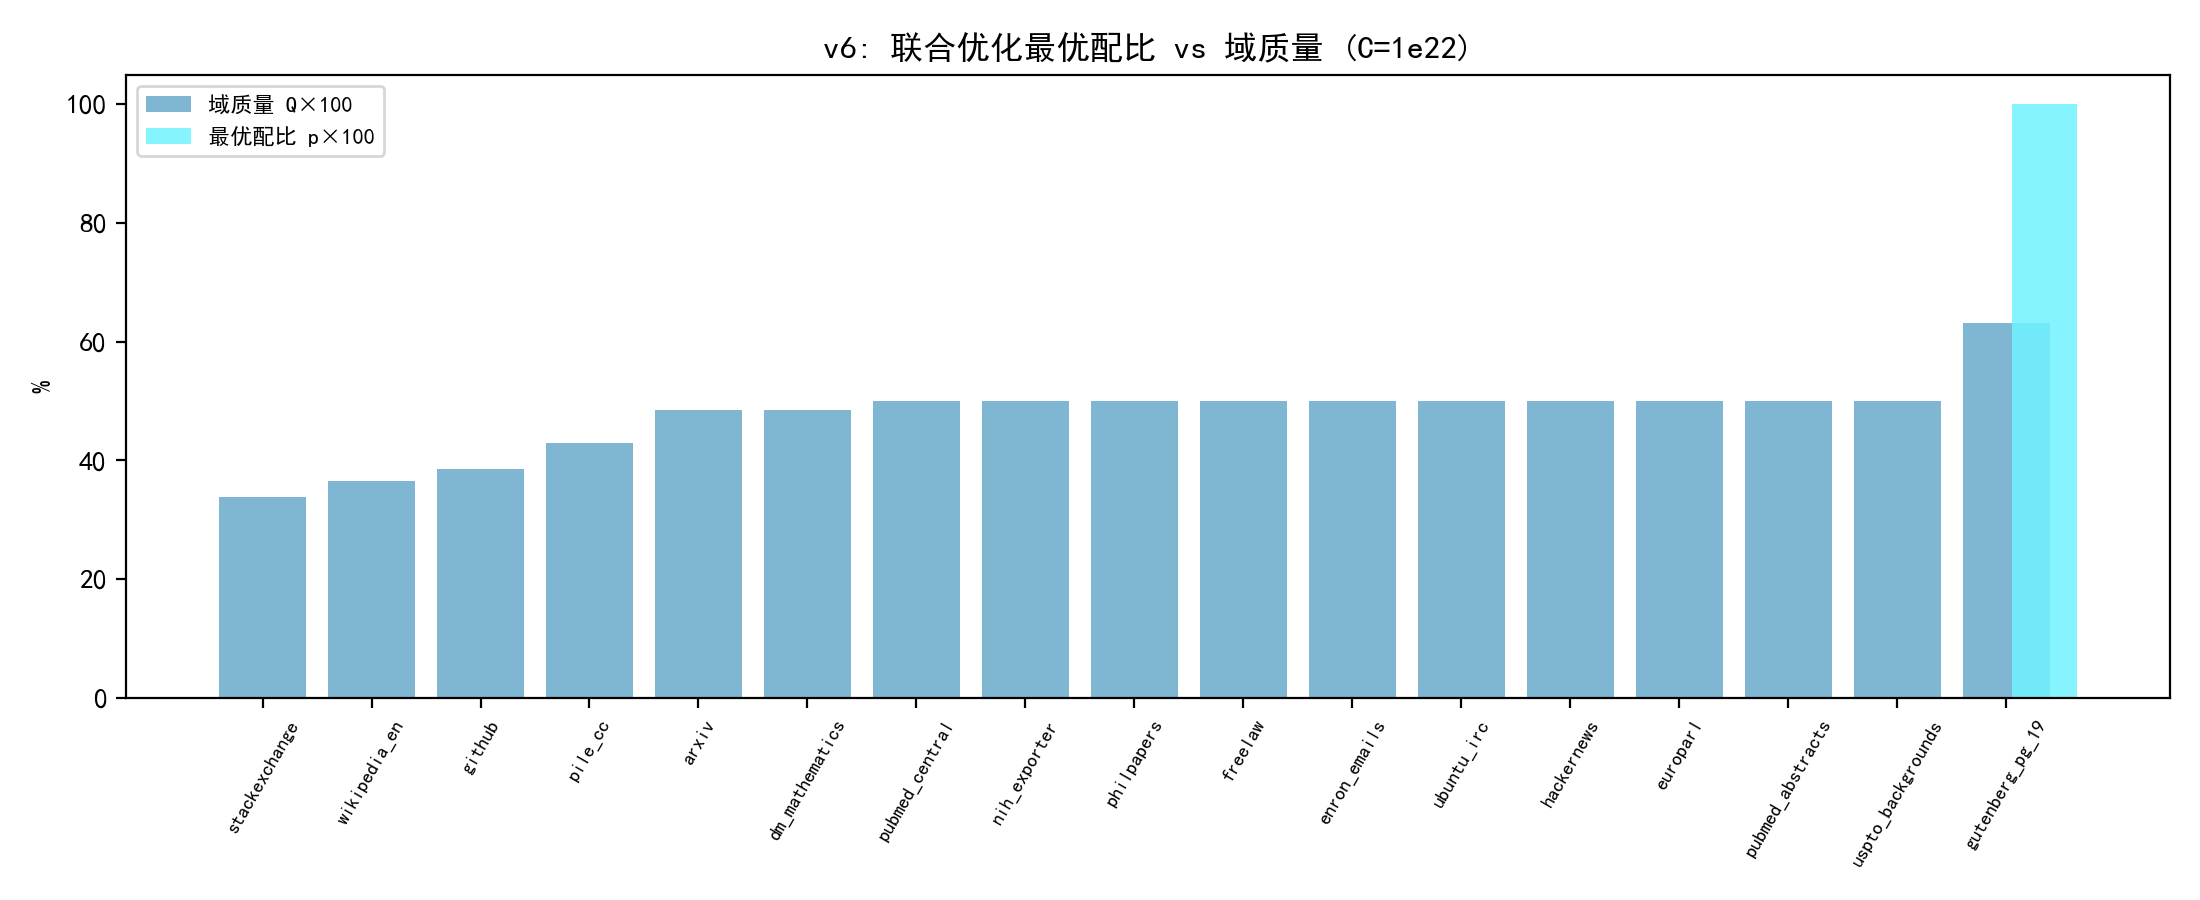
\includegraphics[width=0.9\textwidth]{figures/v6_p3_joint.png}
\caption{联合优化最优配比与域质量对比（$C=10^{22}$）：配比向最高质量域（小说）集中。}
\label{fig:p3_joint_mix}
\end{figure}

\subsubsection{上下文长度内生化}

前述优化将 $L_{\text{ctx}}$ 视为外生参数。本步将其提升为决策变量，并以
C7 架构元数据（40 个开源模型）拟合\textbf{上下文能力收益曲线}：
$\ln S=0.367+0.252\ln N+0.197\ln L_{\text{ctx}}$（$R^2=0.535$），即上下文
长度弹性 $0.197$（约等于参数量弹性的一半）。将收益项 $w\cdot
0.197\ln L_{\text{ctx}}$ 加入目标（$w$ 为收益权重）后联合优化：

\begin{itemize}
\item $w=0$（纯损失口径）：最优 $L_{\text{ctx}}$ 退到下限 512，与
``$L_{\text{ctx}}$ 越长损失越高''的结论一致；
\item $w=1$（实证收益口径）：$C=10^{22}$ 时最优 $L_{\text{ctx}}$ 直达架构
上限 131072（$w\ge0.5$ 时已饱和），注意力份额升至 77\%；
\item 权衡本质：长上下文以训练损失为代价换取能力收益——联合优化比固定
4096 的纯损失高 5.9\%，但总目标（损失减收益）更优。
\end{itemize}

\begin{figure}[htbp]
\centering
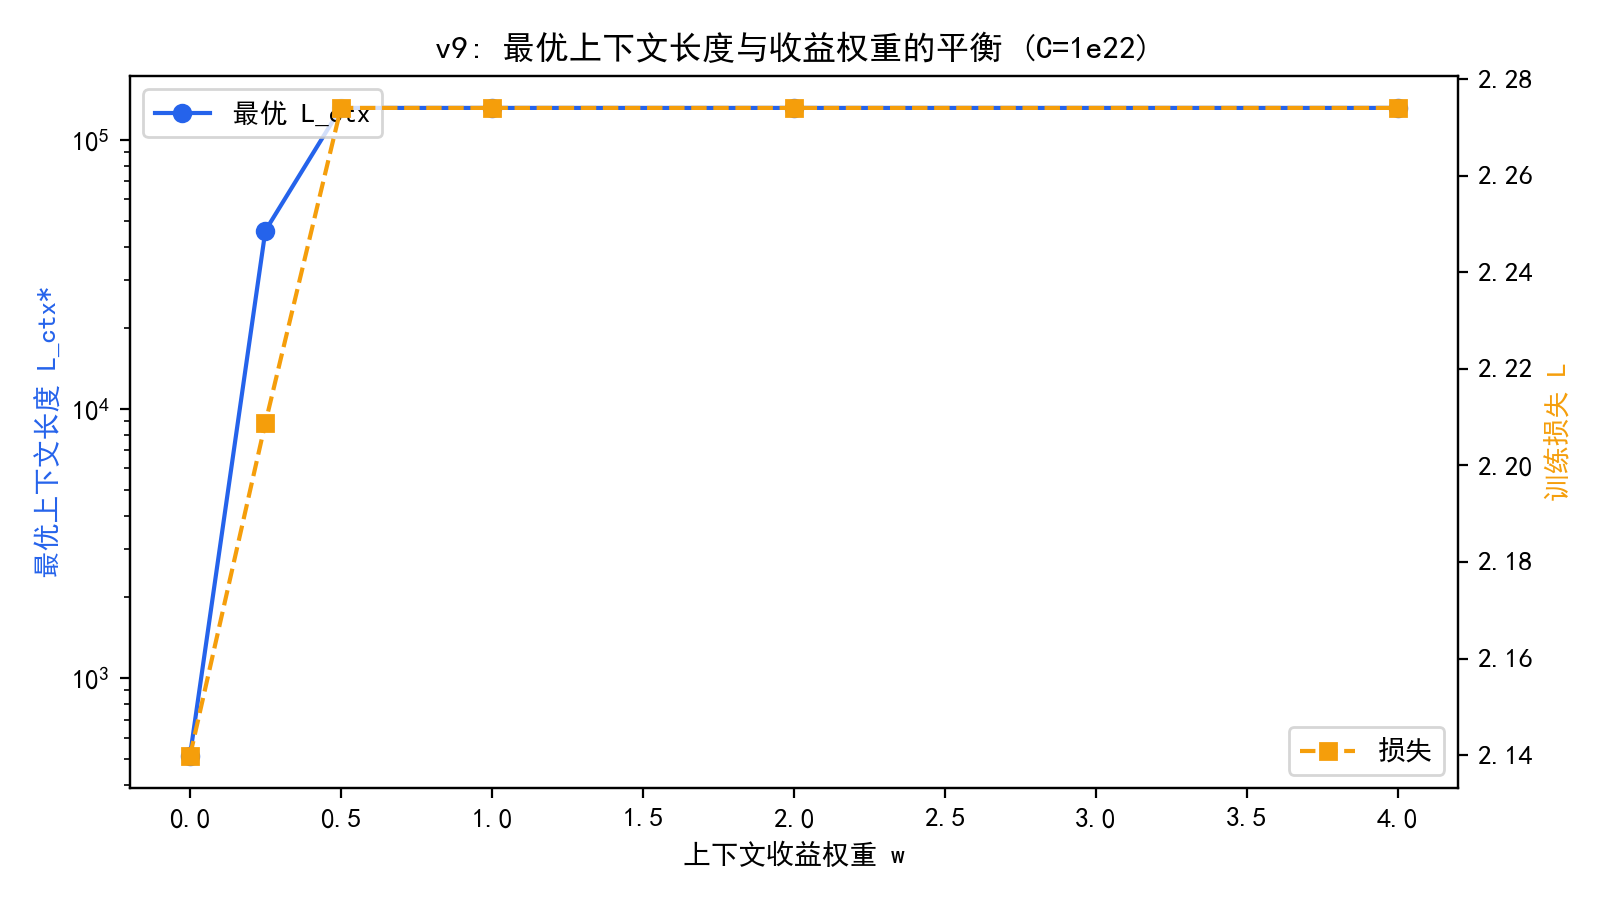
\includegraphics[width=0.8\textwidth]{figures/v9_p3_lctx_inner.png}
\caption{最优上下文长度与收益权重 $w$ 的平衡（$C=10^{22}$）。}
\label{fig:p3_lctx_inner}
\end{figure}

\subsection{小结}

问题三建立了三成本项联合优化模型，得到三档预算最优配置与结构性转移点：
$Q$ 激活阈值约 $10^{18}$ 量级（三种成本函数一致），$10^{22}$ 起质量饱和，
新增预算转向规模；$L_{\text{ctx}}$ 临界点 30000 的注意力--训练份额相等得到
数值验证。配比--质量--算力联合优化进一步表明：语料配比应向高质量域倾斜，
但配比杠杆有限（$\sim$2\%），直接质量投资才是主导途径。上下文长度内生化
（收益弹性 0.197 来自 C7 数据）显示：最优 $L_{\text{ctx}}$ 在纯损失口径下
取下限、在实证收益口径下取架构上限——上下文长度是``能力换损失''的权衡
决策，其最优值取决于收益权重。
